\documentclass[tikz]{standalone}
\usepackage{tikz}
\usetikzlibrary{arrows, calc, patterns, decorations.pathmorphing, fit, positioning, shapes.misc}

\begin{document}
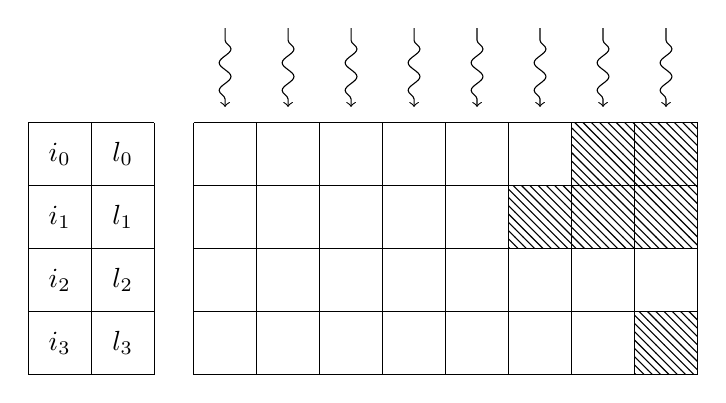
\begin{tikzpicture}
    \def\grid{8}
    \def\pad{5}
    \def\maxCols{8}
    \def\numRows{4}
%     \def\numPost{10}
    \def\rowLengths{7, 8, 5, 6}
    
    \pgfmathtruncatemacro{\matrixWidth}{\grid * \maxCols}
    \pgfmathtruncatemacro{\matrixHeight}{\grid * \numRows}
%     \pgfmathtruncatemacro{\postOffset}{\grid * -2.25}
    \pgfmathtruncatemacro{\lastCol}{\maxCols - 1}
%     \pgfmathtruncatemacro{\lastPost}{\numPost - 1}
    \pgfmathtruncatemacro{\lastRow}{\numRows - 1}
    
    % Draw ragged matrix grid
    \draw[step=\grid mm] (0, 0) grid (\matrixWidth mm, \matrixHeight mm);
    
    % Draw row length grid
    \draw[step=\grid mm, shift={({-\pad mm - (2 * \grid mm)}, 0)}] 
        (0, 0) 
        grid 
        (\grid * 2mm, \matrixHeight mm);
    
%     % Draw postsynaptic neuron grid
%     \draw[step=\grid mm, shift={(\postOffset mm, {-\pad mm - \grid mm})}]
%         (0, 0)
%         grid
%         (\grid * \numPost mm, \grid mm);
        
    % Draw row padding
    \foreach[count=\i] \r in \rowLengths {
        \draw[pattern=north west lines] 
            ({\grid * \r mm}, {(\i - 1) * \grid mm}) 
            rectangle 
            ({\grid * 8mm}, {\i * \grid mm});
    }
    
    % Draw threads
    \foreach \i in {0,...,\lastCol} {
        \draw [<-,decorate,decoration={snake,amplitude=0.75mm,pre length=1mm}]
            ({(\i + 0.5) * \grid mm}, {\matrixHeight mm + 2mm})
            --
            +(0, 10mm);
    }
    
    % Label postsynaptic inputs
%     \foreach \j in {0,...,\lastPost} {
%         \node at ({\postOffset mm + ((\j + 0.5) * \grid mm)}, {-\pad mm - (\grid mm / 2)}){$I_{s_{\j}}$};
%     }
%     
    % Label each presynaptic index and row length
    \foreach \i in {0,...,\lastRow} {
        \node at ({-\pad mm - (1.5 * \grid mm)}, {((\lastRow - \i) + 0.5) * \grid mm}){$i_{\i}$};
        \node at ({-\pad mm - (0.5 * \grid mm)}, {((\lastRow - \i) + 0.5) * \grid mm}){$l_{\i}$};
    }
\end{tikzpicture}
\end{document}